\chapter{2022年「大学物理2」\titlelogo{https://sci.hdu.edu.cn}{HDU}期中试题}
\date{2022年11月12日}{大学物理教学团队}{A0715012}
{未央物理讲师 \href{https://qm.qq.com/q/UPbGudx8cK}{\textbf{Axia}}}
{\qrcode{https://qm.qq.com/q/asJiytD5pC}}{\href{https://qm.qq.com/q/asJiytD5pC}{HDU 物理营}}
{\qrcode{http://weixin.qq.com/r/mhKYgFTEMQlOrRDj90eI}}{\href{http://weixin.qq.com/r/mhKYgFTEMQlOrRDj90eI}{未央学社公众号}}

\section{选择题（每题3分，共27分）}
\begin{choice}{C}[简谐振动]
    一长度为$l$、劲度系数为$k$的均匀轻弹簧分割成长度分别为$l_1$和$l_2$得两部分，且$l_1=nl_2$，$n$为整数.则相应的劲度系数$k_1$和$k_2$为
    \begin{tasks}(2)
        \task $k_1=\frac{kn}{n+1}$，$k_2=k\ab(n+1)$
        \task $k_1=\frac{k\ab(n+1)}{n}$,\ $k_2=\frac{k}{k+1}$
        \task $k_1=\frac{k\ab(n+1)}{n},\ k_2=k\ab(n+1)$
        \task $k_1=\frac{kn}{n+1},\ k_2=\frac{k}{n+1}$
    \end{tasks}
\end{choice}
\begin{solution}*
    弹簧的劲度系数和其长度成反比，所以$k_1=\frac{k\ab(n+1)}{n}$，$k_2=k\ab(n+1)$.\sokka{C}
\end{solution}

\begin{choice}{C}[波的能量]
    一平面简谐波在弹性媒介中传播，在媒质质元从最大位移处回到平衡位置的过程中
    \begin{tasks}(2)
        \task 它的势能转换成动能
        \task 它的动能转换成势能
        \task 它从相邻的一段质元获得能量，其能量逐渐增加
        \task 它把能量传给相邻的一段质元，其能量逐渐减小
    \end{tasks}
\end{choice}
\begin{solution}*
    波在传播过程中介质质元振动的动能和势能同时变化，在从最大位移处运动到平衡位置的过程中动能变大，所以势能也变大，其能量逐渐增加.\sokka{C}
\end{solution}

\begin{paracol}{2}
    \begin{choice}{C}[光程和光程差]
        两相干波源$S_1$和$S_2$相距$\lambda/4$，$S_1$的相位比$S_2$的相位超前$\pi/2$.在$S_1S_2$的连线上两者外侧$P$点两波引起的简谐振动的相位差是
\begin{tasks}(4)
    \task $0$
    \task $\pi/2$
    \task $\pi$
    \task $3\pi/2$
\end{tasks}        
    \end{choice}
\switchcolumn\centering
\vfill
\begin{tikzpicture}
    \draw [very thick,1号色] (-2.4,0)--(2.4,0);
    \length{(0,-0.5)}{(2,-0.5)}{$\frac{1}{4}\lambda$}{(0.5,0)}
    \shade[ball color=red!40] (-2,0) circle (0.05);
    \shade[ball color=red!40] (0,0) circle (0.05);
    \shade[ball color=red!40] (2,0) circle (0.05);
    \node [anchor=south] at (-2,0) {P};
    \node [anchor=south] at (0,0) {$S_1$};
    \node [anchor=south] at (2,0) {$S_2$};
\end{tikzpicture}
\vfill
\end{paracol}
\begin{solution}*
    因传播过程而造成的相位差为$\frac{2\pi\delta}{\lambda}=\frac{2\pi\cdot\lambda/4}{\lambda}=\frac{\pi}{2}$，又因为$S_1$的相位比$S_2$的相位超前$\frac{\pi}{2}$，所以$P$点处两波引起的相位差为$\pi$.\sokka{C}
\end{solution}

\begin{choice}{C}[驻波]
    在弦线上有一简谐波，其表达式是
    \[y_1=2.0\times 10^{-2}\cos{\ab[2\pi\ab(\frac{t}{0.02}-\frac{x}{20})+\frac{\pi}{3}]}\ (\mathrm{SI})\]
    为了在此弦线上形成驻波，并且在$x=0$处为一波节，此弦线上还应有一简谐波，其表达式为
    \begin{tasks}(2)
        \task $y_2=2.0\times 10^{-2}\cos{\ab[2\pi\ab(\frac{t}{0.02}+\frac{x}{20})+\frac{\pi}{3}]}\ (\mathrm{SI})$
        \task $y_2=2.0\times 10^{-2}\cos{\ab[2\pi\ab(\frac{t}{0.02}+\frac{x}{20})+\frac{2\pi}{3}]}\ (\mathrm{SI})$
        \task $y_2=2.0\times 10^{-2}\cos{\ab[2\pi\ab(\frac{t}{0.02}+\frac{x}{20})+\frac{4\pi}{3}]}\ (\mathrm{SI})$
        \task $y_2=2.0\times 10^{-2}\cos{\ab[2\pi\ab(\frac{t}{0.02}+\frac{x}{20})-\frac{\pi}{3}]}\ (\mathrm{SI})$
    \end{tasks}
\end{choice}
\begin{solution}*
    由题意得原点处有$y_1+y_2=A\cos{\ab(\omega t+\frac{\pi}{3})}+A\cos{\ab(\omega t+\varphi)}=0$，得$\varphi=\frac{4\pi}{3}$.\sokka{C}
\end{solution}

\begin{choice}{B}[多普勒效应]
    一机车汽笛频率为$750\mathrm{Hz}$，机车以时速$90$公里远离静止的观察者，观察者听到声音的频率是（空气中声速$340\mathrm{m/s}$）
    \begin{tasks}(4)
        \task $810\mathrm{Hz}$
        \task $699\mathrm{Hz}$
        \task $805\mathrm{Hz}$
        \task $695\mathrm{Hz}$
    \end{tasks}
\end{choice}
\begin{solution}
    已知多普勒效应观察者（Observer）和发射源（Source）的的频率关系为
    \[\nu=\frac{u\pm v_o}{u\mp v_s}\nu_0\]

    $v_o$为观察者速度，接近为$+$，远离为$-$；$v_s$为发射源速度，接近为$-$，远离为$+$.观察者静止，其所听频率为
    \[\nu=\frac{340}{340+25}\times 750\mathrm{Hz}\approx 699\mathrm{Hz}\]

    \sokka{B}
\end{solution}

\begin{choice}{C}[光程和光程差]
    真空中波长为$\lambda$的单色光，在折射率为$n$的均匀透明媒质中，从$A$点沿某一路径传播到$B$点，路径的长度为$l$，$A$、$B$两点光振动的相位差记为$\Delta\phi$，则
    \begin{tasks}(4)
        \task $l=\frac{3\lambda}{2},\ \Delta\phi=3\pi$
        \task $l=\frac{3\lambda}{2n},\ \Delta\phi=3n\pi$
        \task $l=\frac{3\lambda}{2n},\ \Delta\phi=3\pi$
        \task $l=\frac{3n\lambda}{2},\ \Delta\phi=3n\pi$
    \end{tasks}
\end{choice}
\begin{solution}*
    $\Delta\phi=\frac{2\pi\delta}{\lambda}=\frac{2\pi nl}{\lambda}$，将四个选项分别代入后只有C选项符合.\sokka{C}
\end{solution}

\begin{choice}{D}[双缝干涉]
    在双缝干涉实验中，两缝间距离为$d$，双缝与屏幕之间的距离为$D$（$D\gg d$）.波长为$\lambda$的平行单色光垂直照射到双缝上，屏幕上干涉条纹中相邻暗纹之间的距离是
    \begin{tasks}(4)
        \task $\frac{2\lambda D}{d}$
        \task $\frac{\lambda d}{D}$
        \task $\frac{dD}{\lambda}$
        \task $\frac{\lambda D}{d}$
    \end{tasks}
\end{choice}
\begin{solution}*
    由明纹公式$x=k\frac{\lambda D}{d}$得暗纹间距$\Delta x=\frac{\lambda D}{d}$.\sokka{D}
\end{solution}

\begin{choice}{A}[劈尖干涉]
    两块平玻璃构成空气劈形膜，左边为棱边，用单色平行光垂直入射，若上面的平玻璃以棱边为轴，沿逆时针方向做微小转动，则干涉条纹的
    \begin{tasks}(2)
        \task 间隔变小，并向棱边方向平移
        \task 间隔变大，并向远离棱边方向平移
        \task 间隔不变，并向棱边方向平移
        \task 间隔变小，并向远离棱边方向平移
    \end{tasks}
\end{choice}
\begin{solution}*
    旋转过程中空气劈形膜的顶角变大，根据条纹间距公式$\Delta x=\frac{\lambda}{2\theta}$所以条纹间隔变小；每处的光程差增大，所以对应的条纹级数增大，表现为向棱边方向平移.\sokka{A}
\end{solution}

\begin{paracol}{2}
    \begin{choice}{C}[弗琅禾费衍射]
    在如图所示的单缝弗琅禾费衍射装置中，将单缝宽度$a$稍稍变宽，同时使单缝沿$y$轴正方向做微小平移（透镜屏幕位置不动），则屏幕$C$上的中央衍射条纹将
    \begin{tasks}(2)
        \task 变窄，同时向上移
        \task 变窄，同时向下移
        \task 变窄，不移动
        \task 变宽，同时向上移
    \end{tasks}
    \end{choice}
    \switchcolumn\centering
    \vfill
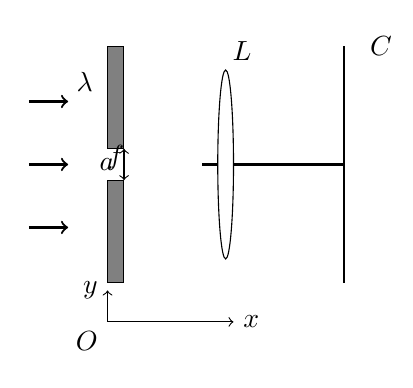
\begin{tikzpicture}
    \filldraw [fill=gray] (0,1.5) rectangle (0.2,0.2);
    \filldraw [fill=gray] (0,-1.5) rectangle (0.2,-0.2);
    \draw [thick] (1.2,0)--(3,0);
    \draw [thick] (3,1.5)--(3,-1.5);
    \filldraw [fill=white] (1.5,0) ellipse (0.1 and 1.2);
    \foreach \y in {0.8,0,-0.8}
    \draw [thick,->,yshift=\y cm] (-1,0)--(-0.5,0);
    \draw [<->] (0,-1.6)--(0,-2)--(1.6,-2);
    \node [anchor=east] at (0,-1.6) {$y$};
    \node [anchor=north east] at (0,-2) {$O$};
    \node [anchor=west] at (1.6,-2) {$x$};
    \length{(1.5,-1.4)}{(3,-1.4)}{$f$}{(0.25,0)}
    \draw [<->] (0,0.2)--(0,-0.2) node [anchor=east,midway] {$a$};
    \node [anchor=south] at (-0.5,0.8) {$\lambda$};
    \node [anchor=south] at (1.5,1.2) {$L$};
    \node [anchor=west] at (3,1.5) {$C$};
\end{tikzpicture}
    \vfill
\end{paracol}
\begin{solution}*
    光线方向不变，所以中央明纹位置不变；根据中央明纹宽度$\Delta x_0=\frac{2\lambda f}{a}$可知单缝宽度增大，中央明纹宽度将变窄.\sokka{C}    
\end{solution}

\section{填空题（共25分）}
\begin{problem}[弹簧振子][3]
一弹簧振子，弹簧的劲度系数为$k$，重物的质量为$m$，则此系统的固有振动周期为\ans{$2\pi\sqrt{m/k}$}.
\end{problem}

\begin{problem}[简谐振动][4]
    一系统做简谐振动，周期为$T$，以余弦函数表达振动时，初相为零.在$0\leq t\leq T/2$范围内，系统在$t=$\ans{$T/8,\ 3T/8$}时刻动能和势能相等.
\end{problem}
\begin{solution}*
    动能等于势能即总能量为势能的$2$倍，$2\cdot\frac{1}{2}kx^2=\frac{1}{2}kA^2$，由此得$x=\pm\frac{\sqrt{2}}{2}A$，对应时刻$t=\frac{1}{8}T,\ \frac{3}{8}T$.
\end{solution}

\begin{problem}[平面简谐波的物理量][4]
    一平面简谐波$y=0.025\cos{\ab(125t-0.37x)}$ (SI).其角频率$\omega=$\ans{$125\mathrm{s}^{-1}$}，波速$u=$\ans{$337.84\mathrm{m/s}$}，波长$\lambda=$\ans{$16.98\mathrm{m}$}.
\end{problem}
\begin{solution}*
    与表达式$y=A\cos\ab(\omega t-2\pi x/\lambda+\varphi)$比对即可.
\end{solution}

\begin{problem}[平面简谐波的波函数][5]
    一平面简谐波沿$Ox$轴正方向传播，波长为$\lambda$，若位于$x=-L_1$的$P_1$处质点的振动方程为$y_1=A\cos\ab(2\pi\nu t+\phi)$，则位于$x=L_2$的$P_2$处质点的振动方程为\ans{$y_2=A\cos\ab[2\pi\nu t-\frac{2\pi\ab(L_2+L_1)}{\lambda}+\phi]$}；与$P_1$处质点振动状态相同的那些点的位置为\ans{$x=-L_1+k\lambda,\ k=0,\pm 1,\pm 2,\cdots$}.
\end{problem}
\begin{solution}
    设波函数为$y=A\cos\ab[2\pi\nu\ab(t-\frac{x}{\lambda\nu})+\varphi_0]$.将$P_1$点坐标$x=-L_1$代入，得
    \[y_1=A\cos\ab[2\pi\nu\ab(t+\frac{L_1}{\lambda\nu})+\varphi_0]\]

    将上式与$P_1$点振动方程比较，得初相$\varphi_0=\phi-\frac{2\pi L_1}{\lambda}$.将$\varphi_0$代入波函数中，得该波的表达式
    \[y=A\cos\ab[2\pi\nu t-\frac{2\pi\ab(x+L_1)}{\lambda}+\phi]\]

    现在令$x=L_2$，得到$P_2$点的振动方程
    \[y_2=A\cos\ab[2\pi\nu t-\frac{2\pi\ab(L_2+L_1)}{\lambda}+\phi]\]

    与点$P_1$处质点振动状态相同的点与$P_1$点的距离应为波长的整数倍，即$x=-L_1+k\lambda,\ k=0,\pm 1,\pm 2,\cdots$.
\end{solution}

\begin{paracol}{2}
    \begin{problem}[平面简谐波的物理量][3]
    一简谐波沿$x$轴正方向传播，$x_1$与$x_2$两点处的振动曲线如图所示.已知$x_2>x_1$且$x_2-x_1<\lambda$，则波从$x_1$点传到$x_2$点所用时间为\ans{$\frac{3}{4}T$}（用简谐波的周期$T$表示）.
    \end{problem}
    \switchcolumn\centering
    \vfill
    \begin{tikzpicture}[scale=0.75]
        \draw [->,thick,](-0.5,0)--(3.5,0) node [anchor=south] {$t$};
        \draw [->,thick](0,-1.2)--(0,1.5) node [anchor=east] {$y$};
        \node [anchor=north east] at (0,0) {$O$};
        \draw[thick,H1] (0,0) sin (0.5,1) cos (1,0) sin (1.5,-1) cos (2,0) sin (2.5,1) cos (3,0);
        \draw[thick] (0,1) cos (0.5,0) sin (1,-1) cos (1.5,0) sin (2,1) cos (2.5,0) sin (3,-1);
        \node [anchor=west,1号色] at (2.5,1) {$x_1$};
        \node [anchor=south west,2号色] at (3,-1) {$x_2$};
        \node [anchor=east] at (0,1) {$A$};
        \node [anchor=north] at (0.5,0) {\scriptsize$T/4$};
        \node [anchor=south] at (1,0) {\scriptsize$T/2$};
    \end{tikzpicture}
    \vfill
\end{paracol}
\begin{solution}*
    简谐波沿$x$轴正方向传播，根据图像很容易判断经过$3T/4$后$x_1$的波形与$x_2$重合.
\end{solution}

\begin{problem}[增透膜][3]
    一束波长为$\lambda=600\mathrm{nm}$的平行单色光垂直入射到折射率为$n=1.33$的透明薄膜上，该膜是放在空气中的.要使反射光得到最大限度的加强，薄膜最小厚度应为\ans{$112.78$}$\mathrm{nm}$.
\end{problem}
\begin{solution}
\begin{itemize}
    \item \textbf{当光从光密介质射向光疏介质时，反射光没有半波损失}.所以两个表面反射光光程差为$\delta=2ne+\frac\lambda2$.
    \item 使反射光干涉相长，即$2ne+\frac\lambda2=k\lambda$. 解得$k=1$时，$e_{\min}=\frac{\lambda}{4n}=112.78\mathrm{nm}$.
\end{itemize}
\end{solution}

\begin{problem}[迈克尔逊干涉仪][3]
    若在迈克尔逊干涉仪的可动反射镜$M$移动$0.620\mathrm{mm}$过程中，观察到干涉条纹移动了$2300$条，则所用光波的波长为\ans{$539.13$}$\mathrm{nm}$.
\end{problem}
\begin{solution}*
    移动带来的光程差满足$\delta=2d=N\lambda$，由此得$\lambda=2d/N=0.644\mathrm{mm}$.
\end{solution}

\section{计算题（共48分）}
\begin{problem}[简谐振动][10]
    一物体质量为$0.25\mathrm{kg}$，在弹性力作用下做简谐振动，弹簧的劲度系数$k=25\mathrm{N/m}$.如果起始振动时具有势能$0.06\mathrm{J}$和动能$0.02\mathrm{J}$，求
    \begin{enumerate}
        \item 振幅.
        \item 动能恰等于势能时的位移.
        \item 经过平衡位置时物体的速度.
    \end{enumerate}
\end{problem}
\begin{solution}
    \begin{enumerate}
        \item 总能量为动能与势能之和，由总能量表达式
        \[E=\frac{1}{2}kA^2=E_k+E_p=0.02\mathrm{J}+0.06\mathrm{J}=0.08\mathrm{J}\eqno\point{3}\]
        得振幅为$A=8\mathrm{cm}$.\point{1}
        \item 动能和势能相等，即总能量为势能的$2$倍，$2\cdot\frac{1}{2}kx^2=\frac{1}{2}kA^2$，由此得$x=\pm\frac{\sqrt{2}}{2}A=\pm 5.66\mathrm{cm}$.\point{3}
        \item 经过平衡位置时系统势能为$0$，总能量与动能相等，$\frac{1}{2}mv^2=0.08\mathrm{J}$，由此得物体的速度为$v=0.8\mathrm{m/s}$.\point{3}
    \end{enumerate}
\end{solution}

\begin{paracol}{2}
    \begin{problem}[简谐振动][5]
        一简谐振动的振动曲线如图所示，求振动方程.
    \end{problem}
    \begin{solution}
        \begin{itemize}
            \item 由图易知振幅$A=0.1\mathrm{m}$.\point{1}
            \item $t=0$时，$x=-5\mathrm{cm},\ v<0$，所以初相$\varphi=\frac{2\pi}{3}$.\point{1}
            \item $t=1$时，$x=0,\ v>0$，此时相位$\varphi=-\frac{\pi}{2}=\omega\cdot 1+\frac{2\pi}{3}$，得角频率$\omega=\frac{5}{6}\pi$.\point{2}
            \item 综上，振动方程为$y=0.1\cos{\ab(\frac{5}{6}\pi t+\frac{2\pi}{3})}$.\point{1}
        \end{itemize}
    \end{solution}
    \switchcolumn\centering
    \vfill
    \begin{tikzpicture}[scale=1.2]
        \draw [->,thick] (-0.5,0)--(3.6,0) node [anchor=south] {$t$};
        \draw [->,thick] (0,-1.5)--(0,1.5) node [anchor=west] {$x$};
        \draw[thick,H1] (0,-0.5) sin (0.4,-1) cos (1,0) sin (1.6,1) cos (2.2,0) sin (2.8,-1) cos (3.4,0);
        \draw [densely dashed] (0,1)--(1.6,1);
        \node [anchor=east] at (0,1) {$10$} node [anchor=south east] at (0,0) {$O$} node [anchor=east] at (0,-0.5) {$-5$} node [anchor=east] at (0,-1) {$-10$} node [anchor=south east] at (1,0) {$1$};
    \end{tikzpicture}
    \vfill
\end{paracol}

\begin{problem}[平面简谐波的波函数][5]
    一振幅为$10\mathrm{cm}$，波长为$200\mathrm{cm}$的简谐横波，沿着一条很长的水平的绷紧弦从左向右行进，波速为$100\mathrm{cm/s}$.取弦上一点为坐标原点，$x$轴指向右方，在$t=0$时原点处质点从平衡位置开始向位移负方向运动.求以SI单位表示的波动表达式（用余弦函数）及弦上任一点的最大振动速度.
\end{problem}
\begin{solution}
    由题意得，角频率$\omega=2\pi\frac{u}{\lambda}=\pi\mathrm{rad/s}$；$t=0$时$x=0$，$v<0$，所以初相$\varphi=\frac{\pi}{2}$.故波动表达式为
    \[y=0.1\cos\ab[\pi\ab(t-x)+\frac{\pi}{2}]\ (\mathrm{SI})\eqno\text{\texttt{(3pt)}}\]
    最大振动速度$v_m=\omega A=0.1\pi\mathrm{m/s}$.\point{2}
\end{solution}

\begin{problem}[光程和光程差][5]
    $S_1,\ S_2$为两平面简谐波相干波源.$S_2$的相位比$S_1$的相位超前$\frac{\pi}{4}$，波长$\lambda=8.00\mathrm{m}$；$S_1,\ S_2$与$P$点的距离分别为$r_1=12.0\mathrm{m},\ r_2=14.0\mathrm{m}$；$S_1$在$P$点引起的振动振幅为$0.30\mathrm{m}$，$S_2    $在$P$点引起的振动振幅为$0.20\mathrm{m}$.求$P$点的合振幅.
\end{problem}
\begin{solution}*
    $P$点相差$\Delta\varphi=\varphi_2-\varphi_1-\frac{2\pi}{\lambda}\ab(r_2-r_1)=-\frac{\pi}{4}$，合振幅为$A=\sqrt{A_1^2+A_2^2+2A_1A_2\cos{\Delta\varphi}}=0.46\mathrm{m}$.
\end{solution}

\begin{problem}[双缝干涉][10]
    薄钢片上有两条紧靠的平行细缝，用波长$\lambda=546.1\mathrm{mm}$的平面光波正入射到钢片上.屏幕距双缝的距离为$D=2.00\mathrm{m}$，测得中央明纹两侧的第五级明纹间的距离为$\Delta x=12.0\mathrm{mm}$.
    \begin{enumerate}
        \item 求两缝间的距离.
        \item 从任一明纹（记作$0$）向一边数到第$20$条明纹，共经过多大距离？
        \item 如果使光波斜入射到钢片上，条纹间距将如何改变？
    \end{enumerate}
\end{problem}
\begin{solution}
    \begin{enumerate}
        \item 由明纹坐标公式$x=\frac{k\lambda D}{a}$得两侧第五级明纹间隔$\Delta x_5=\frac{10\lambda D}{a}$，$a=\frac{10\lambda D}{\Delta x_5}=0.91\mathrm{mm}$.\point{5}
        \item $20$条明纹间距$x_{20}=\frac{20\lambda D}{a}=24\mathrm{mm}$.\point{3}
        \item 斜入射只会使所有明纹对应的光程差同时改变$a\sin{\theta}$，但是相对位置不变，所以条纹间距不变.\point{2}
    \end{enumerate}
\end{solution}

\begin{paracol}{2}
    \begin{problem}[弗琅禾费衍射][5]
    如图所示，设波长为$\lambda$的平面波沿与单缝平面法线成$\theta$角的方向入射， 单缝$AB$的宽度为$a$，观察弗琅禾费衍射.试求出各极小值（即各暗条纹）的衍射角$\varphi$.
    \end{problem}
    \switchcolumn\centering
    \vfill
\begin{tikzpicture}[decoration={markings,mark=between positions .25 and .8 step 20mm with {\arrow{stealth}}}]
    \filldraw [thick,fill=gray] (0,1.6) rectangle (0.15,0.5);
    \draw [densely dashed,thick] (0,0.5)--(0,-0.5);
    \filldraw [thick,fill=gray] (0,-1.6) rectangle (0.15,-0.5);
    \draw [densely dashed,thick] (-1.5,0)--(2,0);
    \coordinate (b) at (-1.5,0);
    \coordinate (a) at (0,0);
    \coordinate (c) at (-1,-0.4);
    \coordinate (d) at (1.5,0.2);
    \coordinate (e) at (2,0);
    \foreach \a in {-0.5,-0.25,0,0.25,0.5}
    \draw [yshift=\a cm,thick,postaction=decorate,->] (-1,-0.4)--(0,0)--(1.5,0.2);
    \pic["$\theta$", draw=black, very thick, angle
    eccentricity=1.35, angle radius=24]{angle=b--a--c};
    \pic["$\varphi$", draw=black, very thick, angle
    eccentricity=1.35, angle radius=36]{angle=e--a--d};
    \node[anchor=east] at (0,0.6) {$A$} node[anchor=east] at (0,-0.6) {$B$};
\end{tikzpicture}
    \vfill
\end{paracol}
\begin{solution}*
    单缝衍射极小时两条光线的光程差满足$\delta=a\ab(\sin{\theta}-\sin{\varphi})=k\lambda$，由此得各极小值的衍射角$\varphi=\arcsin{\ab(a\sin{\theta}+k\lambda)},\ k=\pm 1,\pm2,\pm3,\cdots$.
\end{solution}

\begin{problem}[牛顿环][8]
    曲率半径为$R$的平凸透镜和平板玻璃之间形成空气薄层，波长为$\lambda$的平行单色光垂直入射，观察反射光形成牛顿环.设平凸透镜与平板玻璃在中心$O$点恰好接触，求
    \begin{enumerate}
        \item 从中心向外数第$k$个明环所对应的空气薄层的厚度$e_k$.
        \item 第$k$个明环的半径$r_k$（用$R$，波长$\lambda$和整数$k$表示，$R\gg e_k$）.
    \end{enumerate}
\end{problem}
\begin{solution}
    \begin{enumerate}
        \item 由第$k$级明环对应的光程差所满足条件$\delta=k\lambda=2e_k+\frac{\lambda}{2}$得空气薄层的厚度$e_k=\frac{2k-1}{4}\lambda$.\point{3}
        \item 由几何关系$R^2=r^2+\ab(R-e_k)^2$略去高阶$e_k^2$得$e_k=\frac{2k-1}{4}\lambda\approx\frac{r_k^2}{2R}$.所以明环半径$r_k=\sqrt{\frac{2k-1}{2}\lambda R}$.\point{5}
    \end{enumerate}
\end{solution}